% cls && pdflatex lab-4-report.tex && cls && pdflatex lab-4-report.tex && start lab-4-report.pdf
\documentclass[12pt, a4paper]{article}
\usepackage[T2A]{fontenc}
\usepackage[utf8]{inputenc}
\usepackage[english,ukrainian]{babel}
\usepackage{amsmath, amssymb}
\usepackage{verbatim}

\usepackage[top = 2 cm, left = 1 cm, right = 1 cm, bottom = 2 cm]{geometry}

\usepackage{float, graphicx}
\usepackage{amsthm}
\newtheorem{lemma}{Лема}
\newtheorem*{lemma*}{Лема}
\newtheorem{theorem}{Теорема}
\newtheorem*{theorem*}{Теорема}
\newtheorem{definition}{Визначення}
\newtheorem*{definition*}{Визначення}
\theoremstyle{definition}
\newtheorem{remark}{Зауваження}
\newtheorem*{remark*}{Зауваження}
\newtheorem{example}{Приклад}
\newtheorem*{example*}{Приклад}
\newtheorem{problem}{Задача}
\newtheorem*{problem*}{Задача}
\newtheorem{solution}{Розв'язок}
\newtheorem*{solution*}{Розв'язок}
\newtheorem{corollary}{Наслідок}
\newtheorem*{corollary*}{Наслідок}

\newcommand{\NN}{\mathbb{N}}
\newcommand{\RR}{\mathbb{R}}
\newcommand{\CC}{\mathbb{C}}
\newcommand{\HH}{\mathcal{H}}
\newcommand{\Min}{\displaystyle\min\limits}
\newcommand{\Max}{\displaystyle\max\limits}
\newcommand{\Sup}{\displaystyle\sup\limits}
\newcommand{\Sum}{\displaystyle\sum\limits}
\newcommand{\Prod}{\displaystyle\prod\limits}
\newcommand{\Int}{\displaystyle\int\limits}
\newcommand{\Iint}{\displaystyle\iint\limits}
\newcommand{\Lim}{\displaystyle\lim\limits}

\newcommand*\diff{\mathop{}\!\mathrm{d}}

\renewcommand{\bf}[1]{\textbf{#1}}
\renewcommand{\epsilon}{\varepsilon}
\renewcommand{\phi}{\varphi}

\DeclareMathOperator{\signum}{sign}
\DeclareMathOperator{\diam}{diam}
\DeclareMathOperator{\rang}{rang}
\DeclareMathOperator{\const}{const}
\DeclareMathOperator{\cond}{cond}
\DeclareMathOperator{\diagonal}{diag}

\numberwithin{equation}{section}

\setlength\parindent{0pt}
\allowdisplaybreaks

\newcommand{\cover}[2]{
\begin{center}
\hfill \break
	Міністерство освіти та науки України \\
	Київський національний університет імені Тараса Шевченка \\ 
	Факультет комп'ютерних наук та кібернетики \\
	Кафедра обчислювальної математики
\end{center}

\vfill 

\begin{center}
	\large{
		Звіт до лабораторної роботи №{#1} на тему: \\ 
		``{#2}''
	}
\end{center}

\vfill 

\begin{flushright}
	Виконав студент групи ОМ-3 \\
	Скибицький Нікіта
\end{flushright}

\vfill 

\begin{center}
    Київ, 2018 
\end{center}

\thispagestyle{empty} 
\newpage
}

\begin{document}

\cover{4}{Інтерполяційні поліноми}

\section{Постановка задачі}

Функція $f(x) = \frac12(|x-4|+|x+4|)$ задана на дискретній множині точок (сітці), які належать проміжку $[-5,7]$. \\

Потрібно:
\begin{enumerate}
	\item Побудувати інтерполяційний поліном Ньютона $P_n (x)$ (величина $n$ може змінюватися) за множиною:
	\begin{enumerate}
		\item Рівновіддалених вузлів.
		\item Чебишовських вузлів.
	\end{enumerate}
	\item Побудувати графіки:
	\begin{enumerate}
		\item $f(x)$, $P_n(x)$;
		\item $f(x)-P_n (x)$, $\omega_n (x)= \Prod_{i=0}^n (x-x_i)$;
	\end{enumerate}
	для обох сіток. Пояснити отриманий результат.
	\item Методом оберненої інтерполяції знайти наближене значення точки (їх може бути декілька)$x_*$, в якій $f(x_*)=y_*$, де $y_*=\Min_{[a,b]}f(x)+\frac23\left(\Max_{[a,b]}f(x)-\Min_{[a,b]}f(x)\right)$.
\end{enumerate}

\section{Теоретична частина}

\subsection{Інтерполяційний поліном Ньютона}

Запишемо формулу Лагранжа інтерполяційного багаточлена
\begin{equation}
    \label{eq:6.15}
    L_n(x) = \Sum_{i=0}^n f(x_i) \cdot \dfrac{\omega_n(x)}{(x-x_i)\cdot \omega_n'(x_i)},
\end{equation}
де $\omega_n(x) = \Prod_{j=0}^n (x-x_j)$. \\

Позначимо $\Phi_j(x) = L_j(x) - L_{j-1}(x)$. Тоді, оскільки
\[ L_n(x) = L_0(x) + (L_1(x) - L_0(x)) + \ldots + (L_n(x) - L_{n-1}(x)), \]
\[ L_j(x_i) = L_{j-1}(x_i) = f(x_i), \quad i = \overline{0,j-1},\]
то
\begin{equation}
    \label{eq:6.16}
    \Phi_j(x_i) = A_j \cdot (x - x_0) \cdot \ldots \cdot (x - x_{j-1}),
\end{equation}
де $A_j$ визначається з умови $\Phi_j(x_j) = L_j(x_j) - L_{j-1}(x_j) = f(x_j) - L_{j-1}(x_j)$. Звідси
\[ \Phi_j(x) = \dfrac{f(x_j)-L_{j-1}(x_j)}{(x_j-x_0)\cdot\ldots\cdots(x_j-x_{j-1})}\cdot(x-x_0)\cdot\ldots\cdot(x-x_j).\] 

Тоді
\begin{multline*}
    A_j = \dfrac{f(x_j)-L_{j-1}(x_j)}{(x_j-x_0)\cdot\ldots\cdots(x_j-x_{j-1})} = \dfrac{f(x_j)}{(x_j-x_0)\cdot\ldots\cdots(x_j-x_{j-1})} - \\
    - \Sum_{i=0}^{j-1} \dfrac{f(x_i)}{(x_i-x_0)\cdot\ldots\cdot(x_i-x_{i-1})\cdot(x_i-x_{i+1})\cdot\ldots\cdot(x_i-x_{j-1})\cdot(x_j-x_i)} = \\
    = \dfrac{f(x_j)}{(x_j-x_0)\cdot\ldots\cdots(x_j-x_{j-1})} + \Sum_{i=0}^{j-1} \dfrac{f(x_i)}{(x_i-x_0)\cdot\ldots\cdot(x_i-x_j)} =  \\
    = \Sum_{i=0}^j \dfrac{f(x_i)}{(x_i-x_0)\cdot\ldots\cdot(x_i-x_{i-1})\cdot(x_i-x_{i+1})\cdot\ldots\cdot(x_i-x_j)} = f(x_0;\ldots;x_j).
\end{multline*}
Звідси маємо інтерполяційну формулу Ньютона вперед ($x_0 \to x_n$):
\begin{equation}
    \label{eq:6.17}
    L_n(x) = f(x_0) + f(x_0;x_1) \cdot (x-x_0) + \ldots + f(x_0;\ldots;x_n) \cdot (x-x_0) \cdot \ldots \cdot (x-x_{n-1}).
\end{equation}

Аналогічно, інтерполяційна формула Ньютона назад ($x_n\to x_0$):
\begin{multline}
    \label{eq:6.18}
    L_n(x) = f(x_n) + f(x_n;x_{n-1}) \cdot (x-x_n) + \ldots \\
    \ldots + f(x_n;\ldots;x_0) \cdot (x-x_n) \cdot \ldots \cdot (x-x_1).
\end{multline}

Маємо рекурсію за степенем багаточлена 
\[ L_n(x) = L_{n-1}(x) + f(x_0;\ldots;x_n)\cdot(x-x_0)\cdot\ldots(x-x_1).\]

Звідси \[L_n(x) = f(x_0) + (x-x_0)\cdot(f(x_0;x_1)+(x-x_1)\cdot(\cdots+(x-x_{n-1})\cdot f(x_0;x_1;\ldots;x_n)))\] і цю формулу розкриваємо починаючи з середини (це аналог схеми Горнера обчислення значення багаточлена). \\

Введемо нову формулу для похибки інтерполювання. Для $x \ne x_i$, $i = \overline{0,n}$ розглянемо розділену різницю
\[ f(x;x_0;\ldots;x_n) = \dfrac{f(x)}{(x-x_0)\cdot\ldots\cdot(x-x_n)} + \Sum_{k=0}^n \dfrac{f(x_k)}{\Prod_{i\ne k}(x-x_i)}.\]

Звідси
\begin{multline*}
    f(x) = f(x_0) \cdot \dfrac{(x-x_1)\cdot\ldots\cdot(x-x_n)}{(x_0-x_1)\cdot\ldots\cdot(x_0-x_n)} + \ldots + f(x_n) \cdot \dfrac{(x-x_1)\cdot\ldots\cdot(x-x_n)}{(x_n-x_1)\cdot\ldots\cdot(x_n-x_{n-1})} + \\
    + f(x;x_0;\ldots;x_n)\cdot(x-x_0)\cdot\ldots\cdot(x-x_n)=L_n(x)+f(x;x_0;\ldots;x_n)\cdot\omega_n(x).
\end{multline*}

Тоді похибка має вигляд
\begin{equation}
    \label{eq:6.19}
    r_n(x) = f(x) - L_n(x) = f(x;x_0;\ldots;x_n)\cdot\omega_n(x).
\end{equation}
Це нова форма для залишкового члена.\\

Порівнюючи з формулою залишкового члена в пункті (6.3), маємо
\[ f(x;x_0;\ldots;x_n) = \dfrac{f^{(n+1)}(\xi)}{(n+1)!},\]
що доводить останню властивість розділених різниць. \\

Нехай маємо сітку рівновіддалених вузлів: $x_i = a + i h$, $h = \frac{b-a}{n}$, $i = \overline{0, n}$, $x_0 = a$, $x_n = b$. Розначимо $\Delta f_0 = f_1 - f_0$, $\Delta^2f_0 = \Delta f_1 - \Delta f_0 = f_2 - 2 f_1 + f_0$, $\ldots$ -- скінченні різниці. Запишемо формули Ньютона у нових позначеннях:
\[ L_n(x) = L_n(x_0 + t h) = f_0 + t \Delta f_0 + \ldots + \dfrac{t\cdot(t-1)\cdot(t-n+1)}{n!}\cdot \Delta^n f_0, \quad t = \dfrac{x-x_0}{h}.\]

Це інтерполяційна формула Ньютона вперед по рівновіддалених вузлах.

\subsubsection{Чебишовські вузли}

\[ x_m = \dfrac{(b-a)\cos\left(\dfrac{2m+1}{2n}\right)\pi+a+b}{2}, \quad m=\overline{0,n-1}.\]
 
\subsubsection{Рівновіддалені вузли}

\[ x_m = a + n \cdot \dfrac{b-a}{n-1}, \quad m=\overline{0,n-1}.\]

\subsection{Метод оберненої інтерполяції}

\begin{figure}[H]
	\centering
	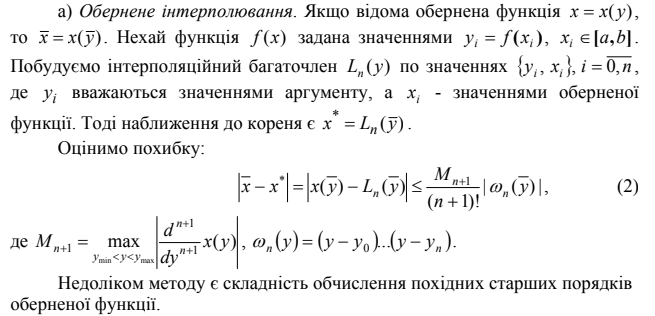
\includegraphics[width=\linewidth]{inverse.png}
\end{figure}

\section{Практична частина}

Покажемо наочні результати для значення $n = 13$, хоча запрограмований алгоритм дає змогу отримати результати $\forall n \in NN$

\[ f(x) = \dfrac12(|x-4|+|x+4|).\]

\subsection{Інтерполяційний поліном Ньютона}
	
\subsubsection{Рівновіддалені вузли}

Для $n = 11$ отримаємо такі вузли:
\begin{table}[H]
	\centering
	\begin{tabular}{|c|c|c|c|c|}
	\hline
	$x_0$ & $x_1$ & $x_2$ & $x_3$ & $x_4$ \\ \hline
	$-5$ & $-2$ & 1 & 4 & 7 \\ \hline
	\end{tabular}
\end{table}

Отримана програма дає такі результати для рівновіддалених вузлів на заданому відрізку

\[P_n(x) = x^5 - x^4 - 24x^3 + 62 x^2 + 139 x - 98.\]

\subsubsection{Чебишовські вузли}
Для $n = 5$ отримаємо такі вузли:
\begin{table}[H]
	\centering
	\begin{tabular}{|c|c|c|c|c|}
	\hline
	$x_0$ & $x_1$ & $x_2$ & $x_3$ & $x_4$\\ \hline
	$-4.7063$ & $-2.5267$ & 1. & 4.5267 & 6.7063 \\ \hline
	\end{tabular}
\end{table}

\[P_n(x) = x^5 - 4.9738 x^4 + 123.667 x^2 + 284.23 x - 352.197.\]

Потрібно зазначити, що коефіцієнти при відповідних степенях зазначені з точністю $\epsilon = 10^{-4}$ біля нуля, тобто якщо $|a_n|<\epsilon$, то $a_n$ береться рівним $0$.

\subsection{Графіки многочленів}

\begin{figure}[H]
	\centering
	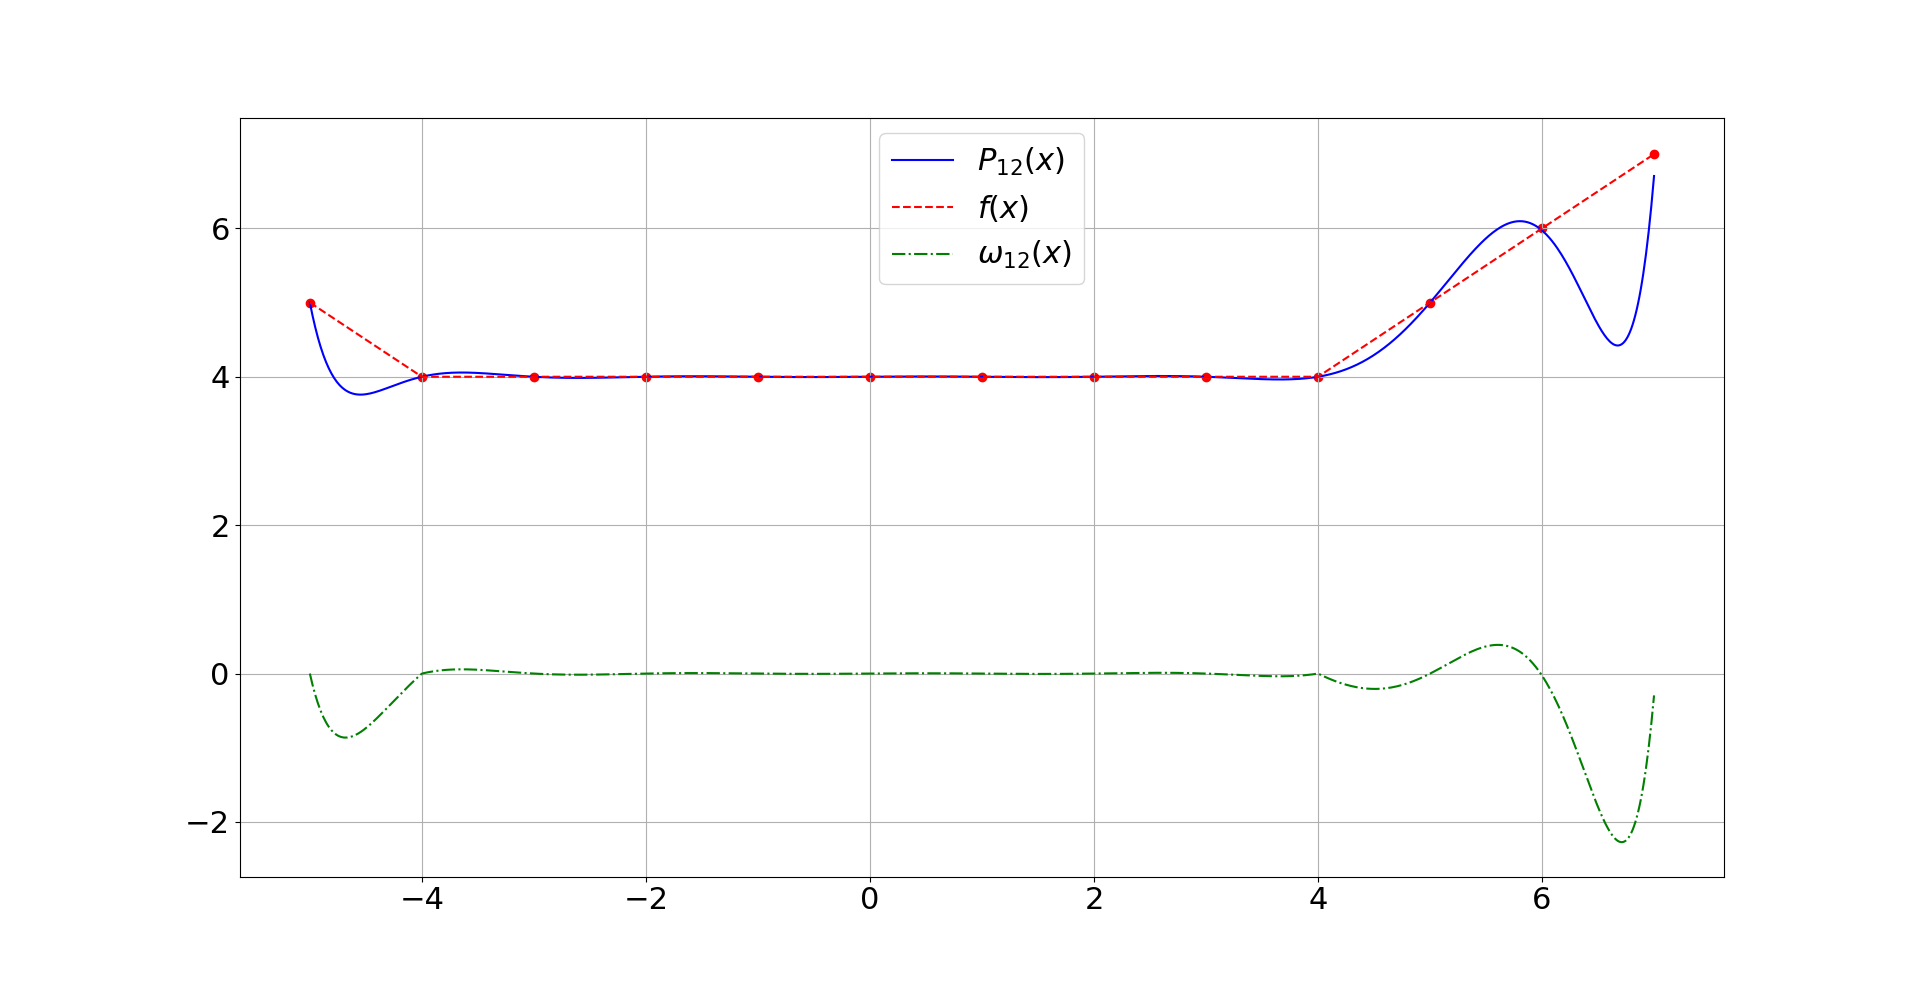
\includegraphics[width=\linewidth]{lab-4-newton.png}
	\caption{Рівновіддалені вузли}
\end{figure}

Проаналізувавши графік побудованого полінома Ньютона по відповідним вузлам, можна сказати що ближче до центру відрізка досягається досить висока точність інтерполяції, проте чим ближче до кінців відрізку, тим більшою стає похибка, при чому вона не є сталою. Поглянувши на графік різниці полінома та початковою функцією, видно, що похибка зростає при прямуванні до країв інтервалу.

\begin{figure}[H]
	\centering
	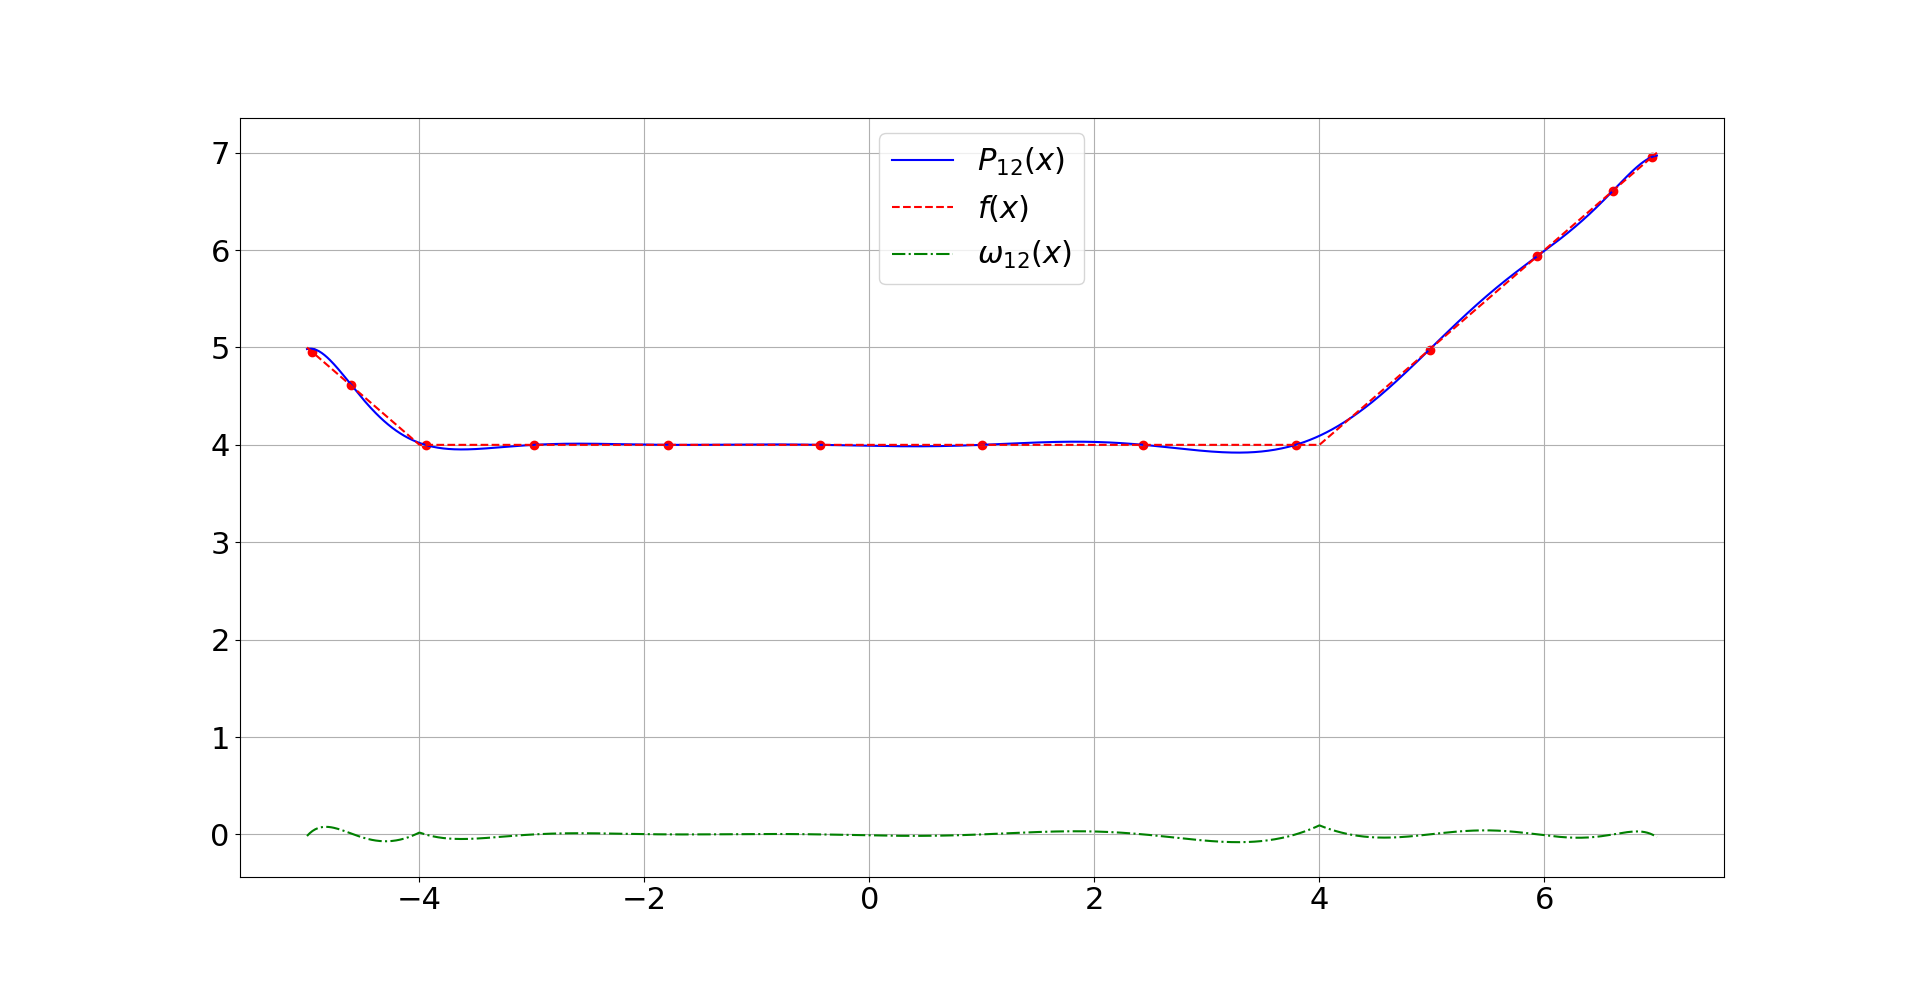
\includegraphics[width=\linewidth]{lab-4-chebyshev.png}
	\caption{Чебишівські вузли}
\end{figure}

Проаналізувавши графік побудованого полінома, можна зробити висновок, що досягнута досить висока точність на всьому інтервалі інтерполювання. Також можна зробити висновок, що чебишовська сітка має таку властивість, як сталість відхилення на всьому інтервалі.

\end{document}
